\documentclass[12pt,aspectratio169]{beamer}

% Use Madrid theme
\usetheme{Madrid}

% Packages
\usepackage{graphicx}
\usepackage{caption}
\setbeamertemplate{navigation symbols}{}
\setbeamertemplate{footline}{}
\setbeamertemplate{footline}[frame number]
\usepackage{amsmath}
\usepackage{color}
\usepackage{caption}
\usepackage{hyperref}
\usepackage{xcolor}
\usepackage{adjustbox}
\usepackage{natbib}
% Title Info
\title{Summer Internship in Computational Nuclear AstroPhysics (SICNAP 2025)}
\subtitle{M.R.P.D. Government College, India}
\author{Yadav Raj Dahal}
%\institute{}
\date{\today}

\begin{document}

% Title slide with logos at the bottom
\begin{frame}
  \titlepage

  % Space before logos
  \vspace{1cm}

  % Logos centered below title
  \begin{center}
    
\includegraphics[height=1cm]{MUSES.png} \hspace{1cm}
    
\includegraphics[height=1cm]{mrpd.png}
  \end{center}
\end{frame}
\begin{frame}{Table of Contents}
\begin{itemize}
    \item Introduction to particle physics
    \item Standard Model overview
    \item Big Bang Theory and Early Universe
    \item QCD Concepts
    \item QCD Phase Diagram
    \item Introduction to the Walecka Model
    \item Mean field approximation
    \item Equation of state in neutron star matter
    \item Conclusion
    
\end{itemize}
\end{frame}

% Example content slide
\begin{frame}[allowframebreaks]{Introduction to Particle Physics}
\hspace{1cm}
Particle physics studies the fundamental constituents of matter and their interactions.

\begin{block}{Fundamental Forces}
\begin{itemize}
    \item \textbf{Strong:} Gluons
    \item \textbf{Electromagnetic:} Photons
    \item \textbf{Weak:} Bosons
    \item \textbf{Gravitational:} Graviton
\end{itemize}
\end{block}
\begin{columns}
    \column{0.4\textwidth}
    \begin{block}{Fundamental Particles}

\begin{itemize}
    \item Matter particles
    \begin{itemize}
        \item \textbf{Quarks:} $u$, $d$, $s$, $c$, $b$, $t$
        \item \textbf{Leptons:} $e^-$, $\mu^-$, $\tau^-$, $\nu_e$, $\nu_\mu$, $\nu_\tau$
    \end{itemize}
    \item Force carriers
    \begin{itemize}
        \item \textbf{Bosons:} photon, $W^\pm$, $Z^0$
    \end{itemize}
    
\end{itemize}
\end{block}
    \column{0.5\textwidth}
    \begin{figure}
    \centering
    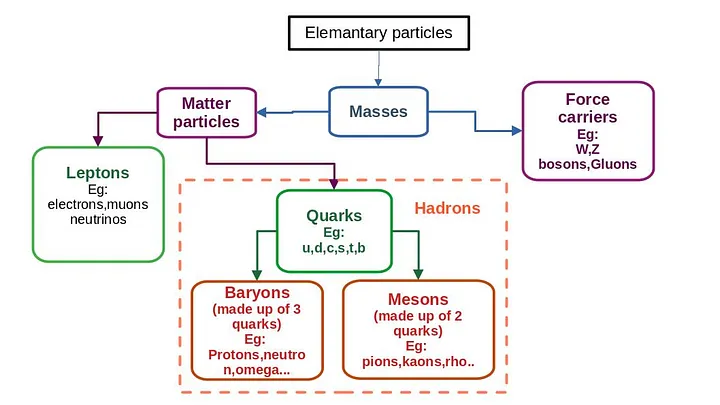
\includegraphics[width= 7cm]{particlephysics.png}
    \caption{Classification of elementary particles\href{https://medium.com/@vivekptl9/particle-physics-an-informal-introduction-d1d63f14ebc8}{\textit{(source)}}}
\end{figure}
\end{columns}

\end{frame}
\begin{frame}{Standard Model Overview}
\begin{columns}
    \column{0.4\textwidth}
    \begin{itemize}
        \item \footnotesize summarizes the interaction of fundamental forces and the structure of atomic particles
        \item Unifies electromagnetic, weak, and strong interactions


    \end{itemize}
    \column{0.6\textwidth}
    \begin{figure}
    \centering
    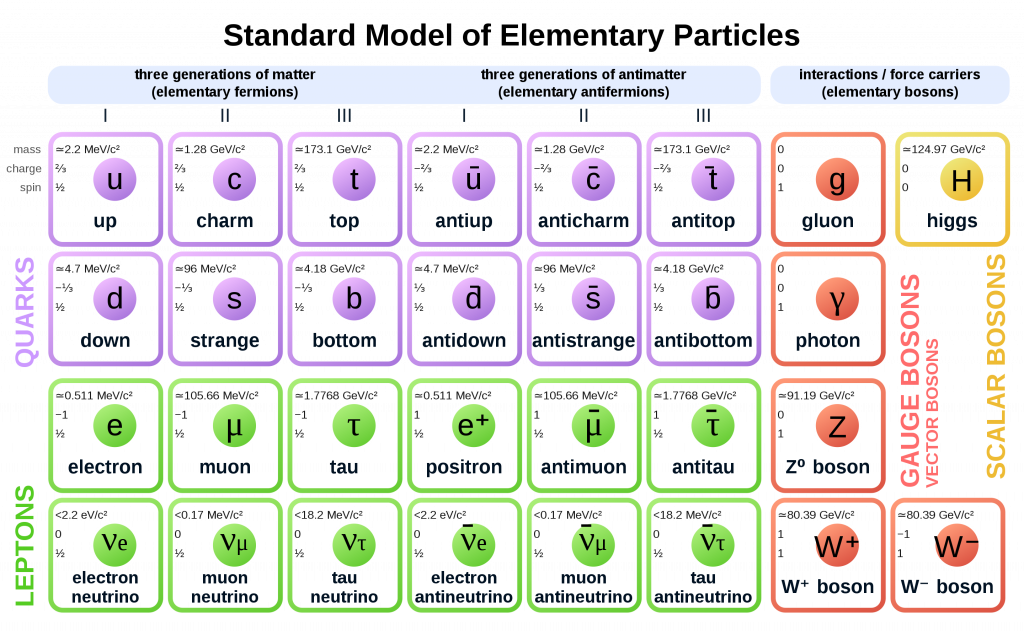
\includegraphics[width=6cm]{standard model.png}
    \caption{Structure of Standard Model\href{https://quantum.lassp.cornell.edu/lecture/elementary_particle_physics}{\textit{(source)}}}
    \end{figure}
\end{columns}
\end{frame}
\begin{frame}{Big bang and early Universe}
\begin{columns}
    \column{0.4\textwidth}
    \begin{itemize}
        \item \footnotesize there was a singularity
        \item explosion and inflation begin
        \item during inflation, gravity separates from other forces
        \item after inflation, temperature began to cool, and matter started to form


    \end{itemize}
    \column{0.6\textwidth}
    \begin{figure}
    \centering
    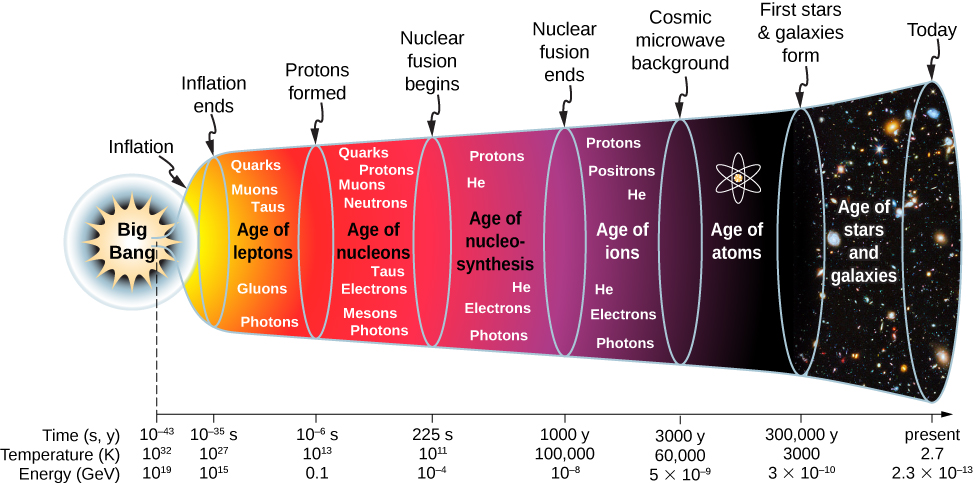
\includegraphics[width=5cm]{bigbang.jpg}
    \caption{evolution of the universe \href{https://phys.libretexts}{\textit{(source)}}}
    \end{figure}
\end{columns}
\end{frame}


\begin{frame}{QCD concepts}
    \begin{itemize}
        \item As the universe continues to expand, strong nuclear force separates from electromagnetic and weak nuclear forces, and eventually weak nuclear force separates from the electromagnetic force
        \item At this time, the universe is a hot soup of quark gluon plasma (QGP), and the physics is governed by quantum chromodynamics(QCD)
        \item QCD is further divided into subregions
        \begin{itemize}
            \item High energy regime$(10^2 GeV)$: Quarks and gluons are asymptotically free
            \item Low energy regime$(10^{-2}GeV)$: Quarks and gluons are confined within the hadrons
        \end{itemize}
 
    \end{itemize}
\end{frame}
\begin{frame}{QCD Phase Diagram}
\begin{columns}

    \column{0.4\textwidth}

    \begin{block}{Main phases}
        \begin{itemize}
            \item \footnotesize In a low temperature to moderate baryonic density, hadrons exist
            \item At high temperature and baryonic density, QGP exists
            \item At low temperature and high baryonic density color superconducting phase exists.
            \item At high temperature and low baryonic density exists a crossover region where quarks and hadrons coexist
        \end{itemize}
    \end{block}
    \column{0.6\textwidth}
    \begin{figure}
    \centering
    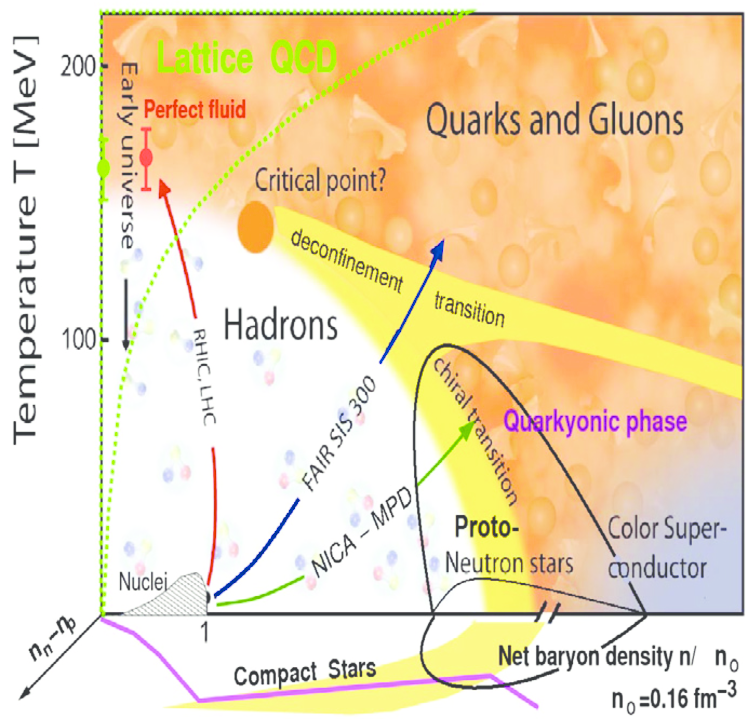
\includegraphics[width=5cm]{QCD-phase-diagram.png}
    \caption{QCD phase diagram \href{https://www.researchgate.net/figure/QCD-phase-diagram_fig5_302061982}{\textit{(source)}}}
    \end{figure}
\end{columns}    
\end{frame}
\begin{frame}{Confinements and Asymptotic Freedom}
    \begin{columns}
    \column{0.4\textwidth}
    \begin{block}{Confinement}
        Quarks and gluons cannot be isolated they are always confined with color color neutral particle(hadrons)
        \begin{itemize}
            \item Free quarks are never observed
        \end{itemize}
    \end{block}
    \column{0.5\textwidth}
    \begin{block}{Asymptotic freedom}
    At very short distances or high temperatures, quarks interact weakly, almost like free particles
    \begin{itemize}
        \item In the early universe, high temperature and low baryonic density quark-gluon interactions weakly form an early ideal fluid
    \end{itemize}
        
    \end{block}
\end{columns}

\end{frame}
\begin{frame}{Introduction to the Walecka Model}
    \begin{itemize}
        \
    \end{itemize}
    \begin{block}{Introduction}
    \begin{itemize}
        \item Relativistic mean field model 
        \item Developed by John D Walecka to describe the properties  of nuclear matter and finite nuclei
        \item Consider only the scaler meson ($\sigma$) (medium range attraction) and the vector meson $\omega^\mu$ (short range repulsion) 
    \end{itemize}
    \end{block}
    
\end{frame}
\begin{frame}{Saturation Properties of Nuclear Matter}
\begin{block}{\textbf{Saturation density($\rho_0$)}}
     \begin{itemize}
        \item \textbf{Number density}:It is defined as the number of baryon per volume
        \item $\rho_0 \approx $$  0.16 fm^{-3} $ 
        \item Indiction of size saturation in atomic nuclei
    \end{itemize}
\end{block}
\begin{block}{\textbf{Binding energy per nucleon}}
    \begin{itemize}
        \item Energy needed to remove one nucleon from nuclear matter
        \item At saturation density$\rho_0$,$B/A \approx -16 MeV$
    \end{itemize}
\end{block}
\begin{block}{\textbf{Compressibility (K)}}
\begin{itemize}
    \item It determines the stifness of EoS
    \item $K  \approx 250- 300MeV$
\end{itemize}
    
\end{block}
   
\end{frame}
\begin{frame}[allowframebreaks]{Lagrangian of the model}
    \begin{block}{Total Lagrangian}
        $\begin{aligned}  \mathcal{L}= & \mathcal{L}_{\text {fermion }}+\mathcal{L}_{\text {scalar }}+\mathcal{L}_{\text {vector }}+\mathcal{L}_{\text {int }} \\ = & \bar{\psi}_i\left(i \gamma^\mu \partial_\mu-m_N\right) \psi_i+g_\sigma^i \bar{\psi}_i \sigma \psi_i-g_\omega^i \bar{\psi}_i \gamma^\mu \omega_\mu \psi_i  \\ & +\frac{1}{2}\left(\partial^\mu \sigma \partial_\mu \sigma-m_\sigma^2 \sigma^2\right)-\frac{1}{4} \omega^{\mu \nu} \omega_{\mu \nu}+\frac{1}{2} m_\omega^2 \omega^\mu \omega_\mu\end{aligned}$\\
         \end{block}
        where 
    $\psi=$ nucleon Dirac field\\
    $\sigma$ = scalar meson field\\
    $\omega^\mu$ = vector meson field\\
    $\omega^{\mu \nu}=\partial^\mu \omega^\nu-\partial^\nu \omega^\mu$
    \\
    $g_\sigma, g_\omega=$ coupling constants\\
    $m_N, m_\sigma, m_\omega=$ masses of nucleon and mesons
   
    \begin{block}{Nucleon/Fermion Term}
        $$
\mathcal{L}_{\text {fermion }}=\bar{\psi}_i\left(i \gamma^\mu \partial_\mu-m_N\right) \psi_
$$
It describes the free Dirac field for the nucleon with the mass $m_N$
    \end{block}
    \begin{block}{Scaler Meson Term $\sigma$}
        $$
\mathcal{L}_{\text {scalar }}=\frac{1}{2}\left(\partial^\mu \sigma \partial_\mu \sigma-m_\sigma^2 \sigma^2\right)
$$
It represents the kinetic and mass terms for the scaler meson $\sigma$
    \end{block}
    \begin{block}{Vector Meson Term $\omega^\mu$}
        $$
\mathcal{L}_{\text {vector }}=-\frac{1}{4} \omega^{\mu \nu} \omega_{\mu \nu}+\frac{1}{2} m_\omega^2 \omega^\mu \omega_\mu
$$
where $\omega^{\mu \nu}=\partial^\mu \omega^\nu-\partial^\nu \omega^\mu$ is the field strength tensor of the vector meson
    \end{block}
    \begin{block}{Interaction Terms}
    $$
\mathcal{L}_{\text {int }}=g_\sigma^i \bar{\psi}_i \sigma \psi_i-g_\omega^i \bar{\psi}_i \gamma^\mu \omega_\mu \psi_i
$$
Above terms describe interactions between nucleons and the scaler/vector mesons
    \end{block}
\end{frame}
\begin{frame}{Equations in the Walecka model}
    Applying Euler-Lagrange equation for each field
   $$
\frac{\partial \mathcal{L}}{\partial \phi}-\partial_\mu\left(\frac{\partial \mathcal{L}}{\partial\left(\partial_\mu \phi\right)}\right)=0
$$
we get
\begin{block}{EOMs}
    \begin{itemize}
        \item Nucleon Field: $$
\left(i \gamma^\mu \partial_\mu-m_N+g_\sigma^i \sigma-g_\omega^i \gamma^\mu \omega_\mu\right) \psi=0
$$
        \item Scaler Field :$$
\left(\partial^\mu \partial_\mu+m_\sigma^2\right) \mathscr{}=g_\sigma \bar{\psi} \psi
$$
        \item Vector Field:$$ \partial_\mu \omega^{\mu\nu} +m^2_\sigma^\nu = g_\sigma \bar{\psi} \gamma^\nu \psi $$
    \end{itemize}
\end{block}
\end{frame}
\begin{frame}{Mean field Approximation}
    In mean field approximation
    \begin{itemize}
        \item Mesons fields are replaced by their expectation values
        \item only time like component survives
    \end{itemize}
    \begin{block}{}
       $\sigma(x) \longrightarrow \bar{\sigma}$\\
       $\omega^\mu (x) \longrightarrow \delta^{\mu0}\omega_0$
 
    \end{block}
    Applying to above EoMs
    \begin{block}{}
        \begin{itemize}
            \item Nucleon field Equation: $\left(i \gamma^\mu \partial_\mu-M^*_i-g_\omega^i \gamma^\mu \omega_\mu\right) \psi=0$ where, $M^*_i =m_N-g_\sigma^i \sigma$ (effective mass)
            \item Scaler meson: $\bar{\sigma} =\frac{g^i_\sigma}{m^2_\sigma}\rho_s$ where, $\rho_s = $scaler density
            \item Vector meson: $\bar{\omega}_0 = \frac{g^i_\omega}{m^2_\omega}\rho_B $ where, $\rho_B=$baryon density
        \end{itemize}
    \end{block}
\end{frame}

\begin{frame}{EoS:Energy and Pressure density}
    \begin{block}{Energy Density}
        \begin{align*}
            \varepsilon_B =& \frac{\gamma}{16\pi^2} \left[
k_F E_F (2k_F^2 + M^{*2}) + M^{*4} \ln \left( \frac{k_F + E_F}{M^*} \right)
\right] \\& + \frac{1}{2} m_\sigma^2 \bar{\sigma}^2 + \frac{1}{2} m_\omega^2 \bar{\omega}_0^2
        \end{align*} 
    \end{block}
    \begin{block}{Pressure Density}
        \begin{align*}
    P_B =& \frac{\gamma}{24\pi^2} \left[
k_F E_F \left(k_F^2 - \frac{3}{2} M^{*2} \right) + \frac{3}{2} M^{*4} \ln \left( \frac{k_F + E_F}{M^*} \right)
\right] \\& - \frac{1}{2} m_\sigma^2 \bar{\sigma}^2 + \frac{1}{2} m_\omega^2 \bar{\omega}_0^2   
        \end{align*}
    \end{block}
\end{frame}
\begin{frame}[allowframebreaks]{Application to Neutron Star Matter}
\begin{block}{Particle Content}
    \begin{itemize}
        \item Nucleons: neutrons and protons
        \item Leptons: electrons and muons
    \end{itemize}
\end{block}
\begin{block}{Charge neutral}
    The net charge must vanish\\
    Total charge must vanish $n_p = n_e + n_\mu$
\end{block}
\begin{block}{Beta Equilibrium}
    Weak interaction processes such as $n p + e^- +$ must be in equilibrium\\
    Chemical potential must satisfy $\mu_n = \mu_p + \mu_e$
\end{block}
\begin{block}{leptonic Contributions}
Electrons and muons are modeled as free relativistic fermi gases.Their number densities and energy densities T = 0 are:
\begin{itemize}
    \item $n_l = \frac{k^3_l}{3\pi^3}$
    \item $\epsilon_l = \frac{1}{\pi^2}\int_o^{k_l}\sqrt{k^2 + m^2_l}k^2dk$
    \item $P_l=\frac{1}{3\pi^2}\int_0^{k_l}\frac{k^4 dk}{\sqrt{k^2 + m^2_l}}$
\end{itemize}
\end{block}
\begin{block}{Modified Energy and Pressure density}
   $$\epsilon_{total} = \epsilon + \epsilon_e$$
    $$P_{total} = P_N + P_e$$
    where $\epsilon_N$ and ${P_N}$ are from Walecka Model and $\epsilon_e$ and $P_e$ from lepton Fermi gas expansions
\end{block}

\end{frame}
\begin{frame}{TOV Equation}
\begin{block}{Tolman-Oppenheimer-Volkoff Equation}
It describes the structure of a static, spherically symmetric distribution of matter in general relativity.\\
It governs the balance of gravitational pull and internal pressure in compact stars like neutron stars.
$$ \frac{dP(r)}{dr} = -\frac{G[\epsilon(r)+\frac{P(r)}{c^2}][m(r)+4\pi r^3\frac{P(r)}{c^2}]}{r^2[1-\frac{2Gm(r)}{rc^2}]}$$

\end{block}
\begin{block}{}
    TOV relate macroscopic quantities (mass and radius) to microscopic quantities (pressure and energy density)
\end{block}
\end{frame}
\begin{frame}{Means field vs Chemical potential}
\begin{minipage}[t]{0.48\textwidth}
  \centering
  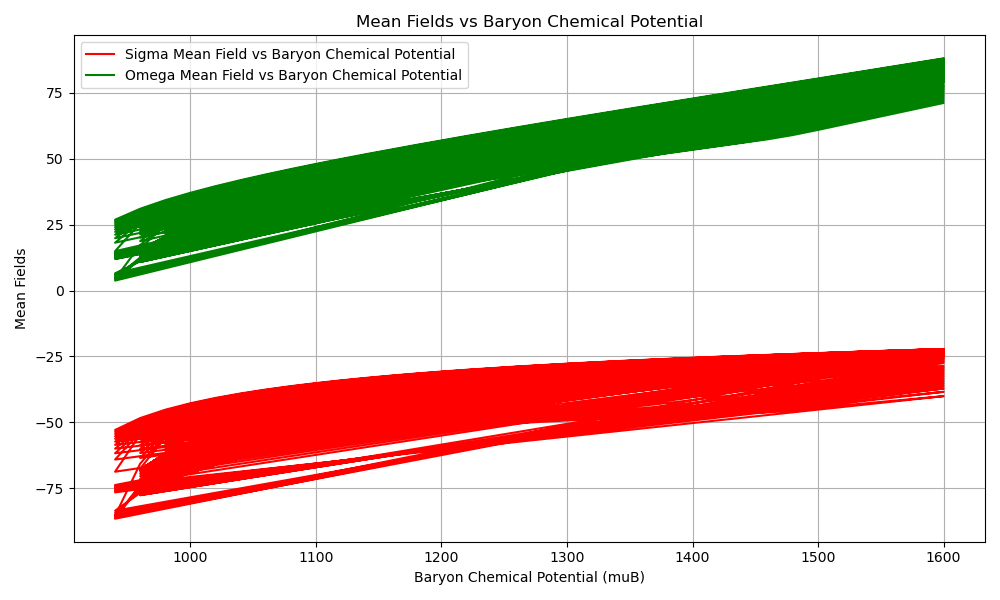
\includegraphics[width=0.9\linewidth]{mean_fields_vs_chemical_potentials1.png}
  %\captionof{figure}{Caption for image 1}
\end{minipage}
\hfill
\begin{minipage}[t]{0.48\textwidth}
  \centering
  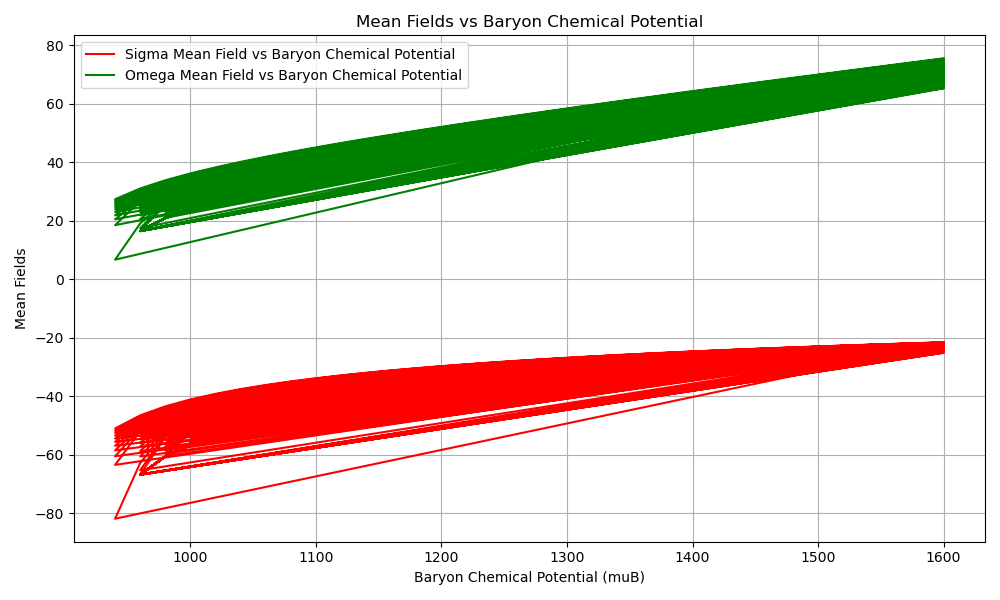
\includegraphics[width=0.9\linewidth]{mean_fields_vs_chemical_potentials2.png}
\end{minipage}

\vspace{0.5cm}

\begin{minipage}[t]{0.48\textwidth}
  \centering
  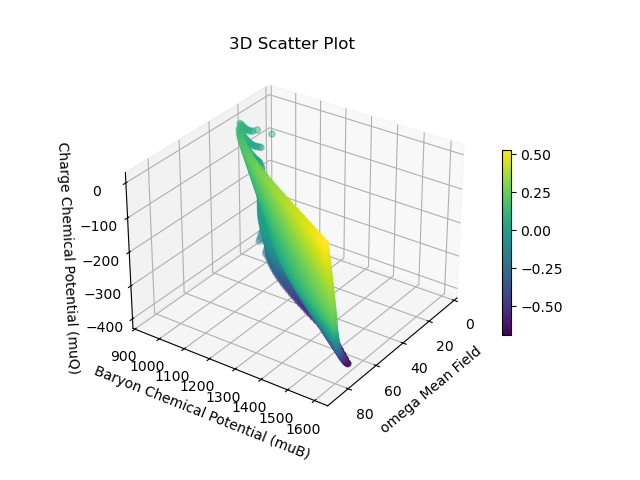
\includegraphics[width=0.9\linewidth]{omega_vs_chemical_potentials1.png}
\end{minipage}
\hfill
\begin{minipage}[t]{0.48\textwidth}
  \centering
  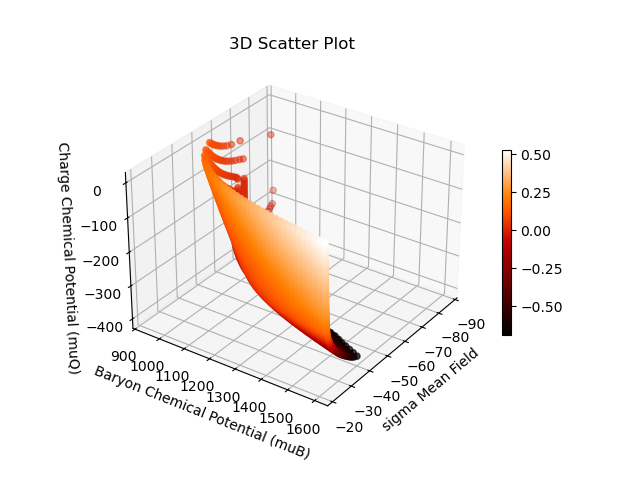
\includegraphics[width=0.9\linewidth]{omega_vs_chemical_potentials2.png}
\end{minipage}

    
\end{frame}

\begin{frame}{Equation of state pressure vs energy density}
\begin{minipage}[t]{0.48\textwidth}
  \centering
  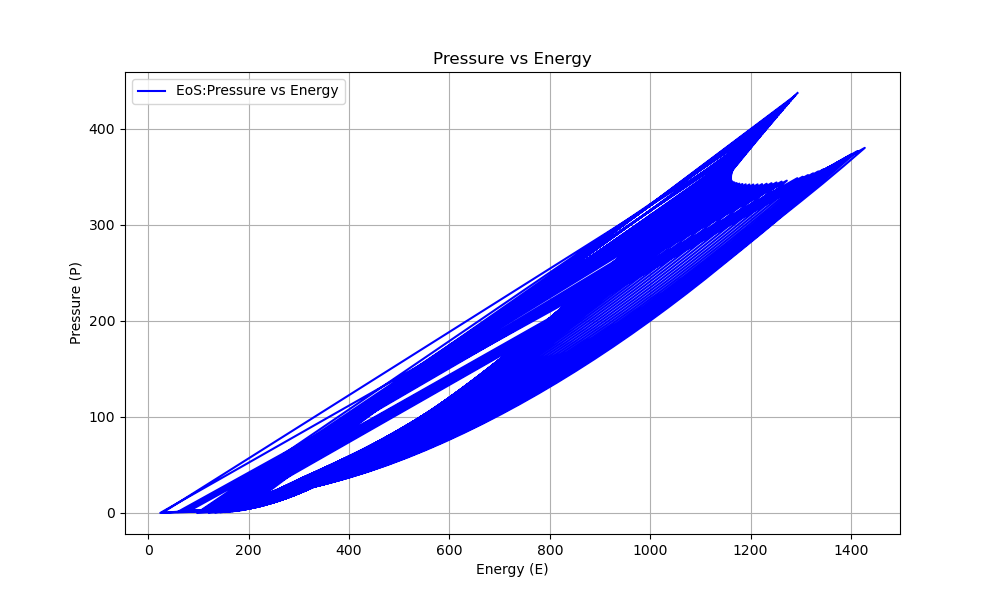
\includegraphics[width=0.9\linewidth]{pressure_vs_energy1.png}
  %\captionof{figure}{Caption for image 1}
\end{minipage}
\hfill
\begin{minipage}[t]{0.48\textwidth}
  \centering
  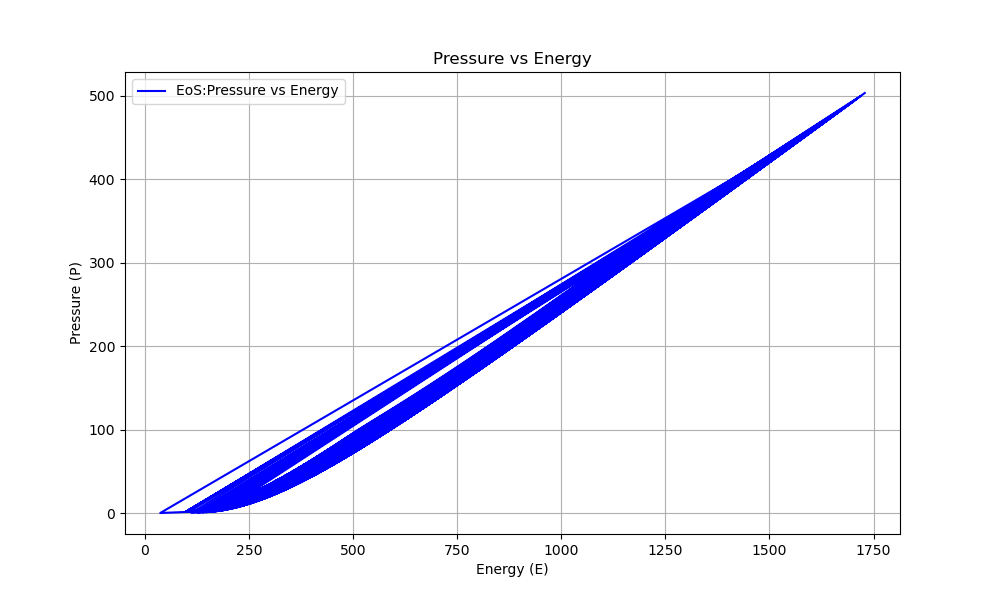
\includegraphics[width=0.9\linewidth]{pressure_vs_energy2.png}
\end{minipage}

\vspace{0.5cm}

\begin{minipage}[t]{0.48\textwidth}
  \centering
  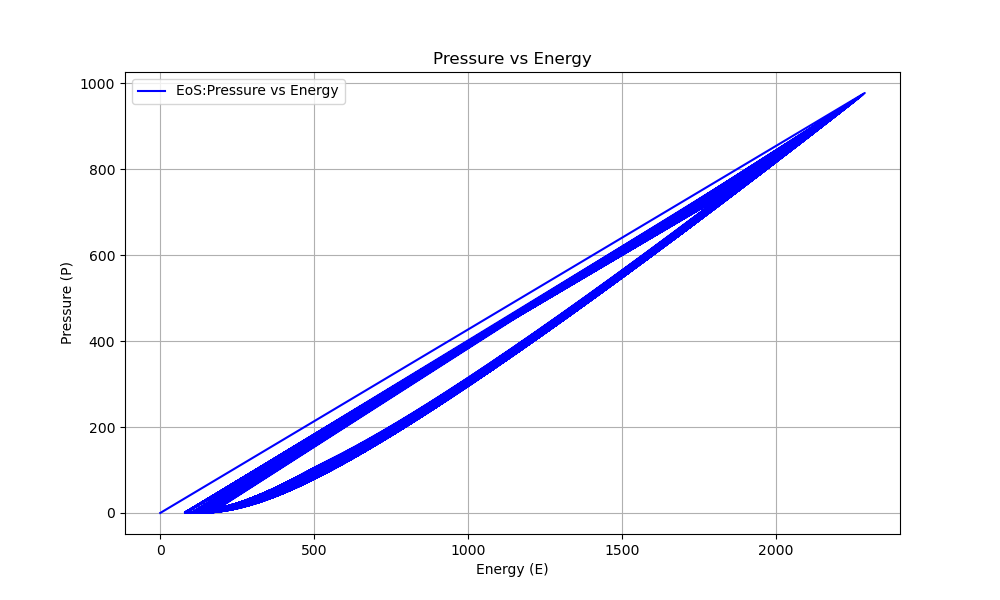
\includegraphics[width=0.9\linewidth]{pressure_vs_energy3.png}
\end{minipage}
\hfill
\begin{minipage}[t]{0.48\textwidth}
  \centering
  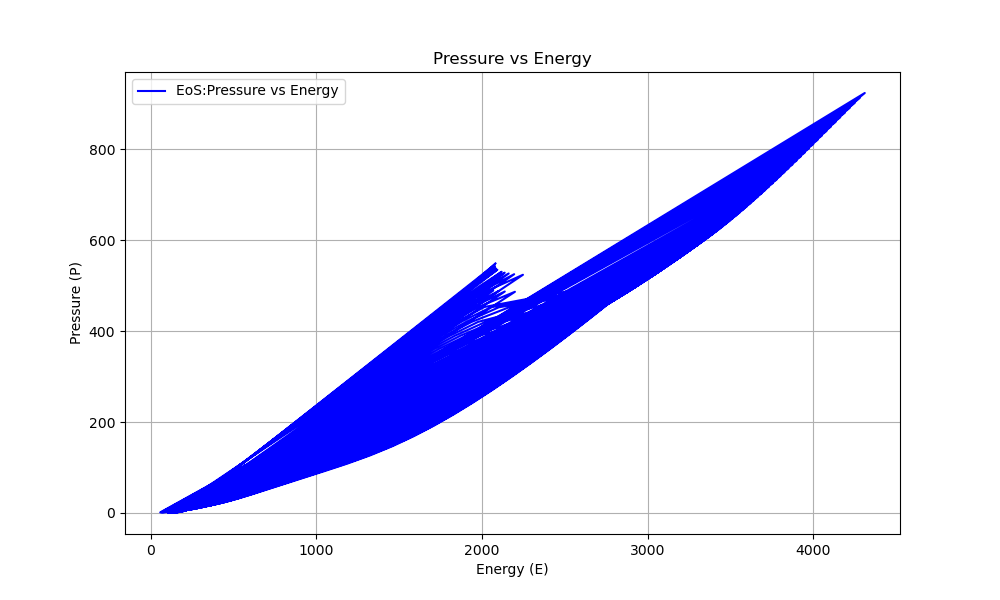
\includegraphics[width=0.9\linewidth]{pressure_vs_energy4.png}
\end{minipage}
    
\end{frame}

\begin{frame}{Mass Radius Curve of a Neutron Star}
MR curve is obtained by plugging the Equation of State (Pressure vs. Energy Density) into the TOV equation\\
\vspace{1cm}
\begin{minipage}[t]{0.48\textwidth}
  \centering
  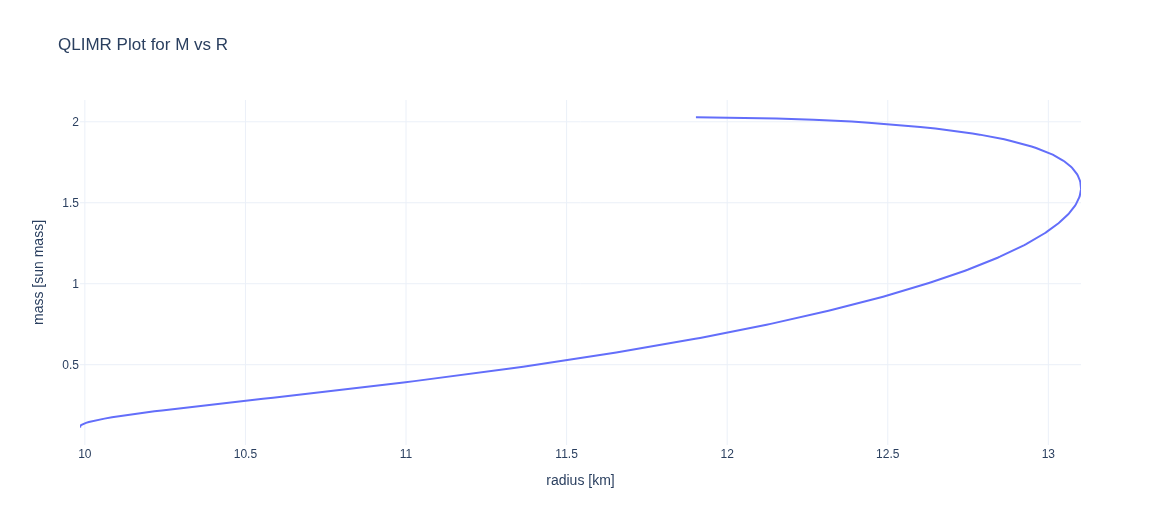
\includegraphics[width=0.9\linewidth]{MR1.png}
\end{minipage}
\hfill
\begin{minipage}[t]{0.48\textwidth}
  \centering
  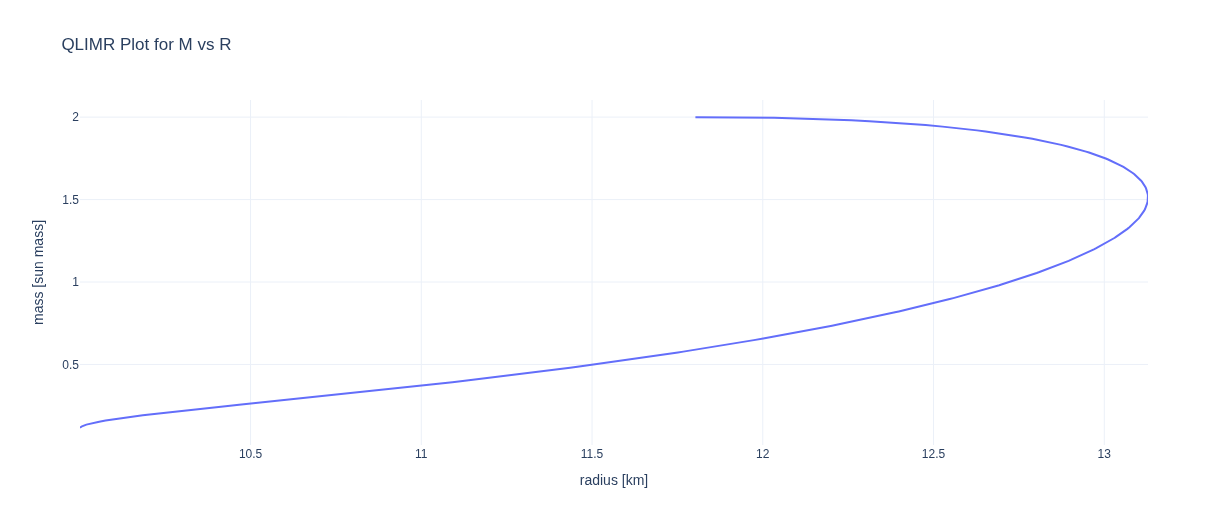
\includegraphics[width=0.9\linewidth]{MR2.png}
\end{minipage}

\vspace{0.5cm}    
\end{frame}
    

\begin{frame}{Conclusion }
\begin{block}{}
Mean Fields ($\sigma, \omega $) vs Baryon Potential($\mu_B$)
\begin{itemize}
    \item Plot shows increasing omega with respect to baryonic chemical potentia,l which means the equation of state will be  more stiff as omega contributes positively to pressure and energy density
\end{itemize}
Pressure vs Energy density
\begin{itemize}
    \item As the energy density increases, the pressure density increases, which indicates that the equation of state is becoming stiff.
\end{itemize}
MR Curve
\begin{itemize}
    \item The maximum mass of a nucleon star is close to two solar masses as the highest point of the curve suggests.
\end{itemize}
\end{block}
\end{frame}

\bibliographystyle{apalike}
\bibliography{references}
\end{document}
